
%% bare_conf.tex
%% V1.3
%% 2007/01/11
%% by Michael Shell
%% See:
%% http://www.michaelshell.org/
%% for current contact information.
%%
%% This is a skeleton file demonstrating the use of IEEEtran.cls
%% (requires IEEEtran.cls version 1.7 or later) with an IEEE conference paper.
%%
%% Support sites:
%% http://www.michaelshell.org/tex/ieeetran/
%% http://www.ctan.org/tex-archive/macros/latex/contrib/IEEEtran/
%% and
%% http://www.ieee.org/

%%*************************************************************************
%% Legal Notice:
%% This code is offered as-is without any warranty either expressed or
%% implied; without even the implied warranty of MERCHANTABILITY or
%% FITNESS FOR A PARTICULAR PURPOSE! 
%% User assumes all risk.
%% In no event shall IEEE or any contributor to this code be liable for
%% any damages or losses, including, but not limited to, incidental,
%% consequential, or any other damages, resulting from the use or misuse
%% of any information contained here.
%%
%% All comments are the opinions of their respective authors and are not
%% necessarily endorsed by the IEEE.
%%
%% This work is distributed under the LaTeX Project Public License (LPPL)
%% ( http://www.latex-project.org/ ) version 1.3, and may be freely used,
%% distributed and modified. A copy of the LPPL, version 1.3, is included
%% in the base LaTeX documentation of all distributions of LaTeX released
%% 2003/12/01 or later.
%% Retain all contribution notices and credits.
%% ** Modified files should be clearly indicated as such, including  **
%% ** renaming them and changing author support contact information. **
%%
%% File list of work: IEEEtran.cls, IEEEtran_HOWTO.pdf, bare_adv.tex,
%%                    bare_conf.tex, bare_jrnl.tex, bare_jrnl_compsoc.tex
%%*************************************************************************

% *** Authors should verify (and, if needed, correct) their LaTeX system  ***
% *** with the testflow diagnostic prior to trusting their LaTeX platform ***
% *** with production work. IEEE's font choices can trigger bugs that do  ***
% *** not appear when using other class files.                            ***
% The testflow support page is at:
% http://www.michaelshell.org/tex/testflow/



% Note that the a4paper option is mainly intended so that authors in
% countries using A4 can easily print to A4 and see how their papers will
% look in print - the typesetting of the document will not typically be
% affected with changes in paper size (but the bottom and side margins will).
% Use the testflow package mentioned above to verify correct handling of
% both paper sizes by the user's LaTeX system.
%
% Also note that the "draftcls" or "draftclsnofoot", not "draft", option
% should be used if it is desired that the figures are to be displayed in
% draft mode.
%
\documentclass[conference]{IEEEtran}
% Add the compsoc option for Computer Society conferences.
%
% If IEEEtran.cls has not been installed into the LaTeX system files,
% manually specify the path to it like:
% \documentclass[conference]{../sty/IEEEtran}





% Some very useful LaTeX packages include:
% (uncomment the ones you want to load)


% *** MISC UTILITY PACKAGES ***
%
%\usepackage{ifpdf}
% Heiko Oberdiek's ifpdf.sty is very useful if you need conditional
% compilation based on whether the output is pdf or dvi.
% usage:
% \ifpdf
%   % pdf code
% \else
%   % dvi code
% \fi
% The latest version of ifpdf.sty can be obtained from:
% http://www.ctan.org/tex-archive/macros/latex/contrib/oberdiek/
% Also, note that IEEEtran.cls V1.7 and later provides a builtin
% \ifCLASSINFOpdf conditional that works the same way.
% When switching from latex to pdflatex and vice-versa, the compiler may
% have to be run twice to clear warning/error messages.






% *** CITATION PACKAGES ***
%
%\usepackage{cite}
% cite.sty was written by Donald Arseneau
% V1.6 and later of IEEEtran pre-defines the format of the cite.sty package
% \cite{} output to follow that of IEEE. Loading the cite package will
% result in citation numbers being automatically sorted and properly
% "compressed/ranged". e.g., [1], [9], [2], [7], [5], [6] without using
% cite.sty will become [1], [2], [5]--[7], [9] using cite.sty. cite.sty's
% \cite will automatically add leading space, if needed. Use cite.sty's
% noadjust option (cite.sty V3.8 and later) if you want to turn this off.
% cite.sty is already installed on most LaTeX systems. Be sure and use
% version 4.0 (2003-05-27) and later if using hyperref.sty. cite.sty does
% not currently provide for hyperlinked citations.
% The latest version can be obtained at:
% http://www.ctan.org/tex-archive/macros/latex/contrib/cite/
% The documentation is contained in the cite.sty file itself.






% *** GRAPHICS RELATED PACKAGES ***
%
\ifCLASSINFOpdf
  % \usepackage[pdftex]{graphicx}
  % declare the path(s) where your graphic files are
  % \graphicspath{{../pdf/}{../jpeg/}}
  % and their extensions so you won't have to specify these with
  % every instance of \includegraphics
  % \DeclareGraphicsExtensions{.pdf,.jpeg,.png}
\else
  % or other class option (dvipsone, dvipdf, if not using dvips). graphicx
  % will default to the driver specified in the system graphics.cfg if no
  % driver is specified.
  % \usepackage[dvips]{graphicx}
  % declare the path(s) where your graphic files are
  % \graphicspath{{../eps/}}
  % and their extensions so you won't have to specify these with
  % every instance of \includegraphics
  % \DeclareGraphicsExtensions{.eps}
\fi
% graphicx was written by David Carlisle and Sebastian Rahtz. It is
% required if you want graphics, photos, etc. graphicx.sty is already
% installed on most LaTeX systems. The latest version and documentation can
% be obtained at: 
% http://www.ctan.org/tex-archive/macros/latex/required/graphics/
% Another good source of documentation is "Using Imported Graphics in
% LaTeX2e" by Keith Reckdahl which can be found as epslatex.ps or
% epslatex.pdf at: http://www.ctan.org/tex-archive/info/
%
% latex, and pdflatex in dvi mode, support graphics in encapsulated
% postscript (.eps) format. pdflatex in pdf mode supports graphics
% in .pdf, .jpeg, .png and .mps (metapost) formats. Users should ensure
% that all non-photo figures use a vector format (.eps, .pdf, .mps) and
% not a bitmapped formats (.jpeg, .png). IEEE frowns on bitmapped formats
% which can result in "jaggedy"/blurry rendering of lines and letters as
% well as large increases in file sizes.
%
% You can find documentation about the pdfTeX application at:
% http://www.tug.org/applications/pdftex





% *** MATH PACKAGES ***
%
%\usepackage[cmex10]{amsmath}
% A popular package from the American Mathematical Society that provides
% many useful and powerful commands for dealing with mathematics. If using
% it, be sure to load this package with the cmex10 option to ensure that
% only type 1 fonts will utilized at all point sizes. Without this option,
% it is possible that some math symbols, particularly those within
% footnotes, will be rendered in bitmap form which will result in a
% document that can not be IEEE Xplore compliant!
%
% Also, note that the amsmath package sets \interdisplaylinepenalty to 10000
% thus preventing page breaks from occurring within multiline equations. Use:
%\interdisplaylinepenalty=2500
% after loading amsmath to restore such page breaks as IEEEtran.cls normally
% does. amsmath.sty is already installed on most LaTeX systems. The latest
% version and documentation can be obtained at:
% http://www.ctan.org/tex-archive/macros/latex/required/amslatex/math/





% *** SPECIALIZED LIST PACKAGES ***
%
%\usepackage{algorithmic}
% algorithmic.sty was written by Peter Williams and Rogerio Brito.
% This package provides an algorithmic environment fo describing algorithms.
% You can use the algorithmic environment in-text or within a figure
% environment to provide for a floating algorithm. Do NOT use the algorithm
% floating environment provided by algorithm.sty (by the same authors) or
% algorithm2e.sty (by Christophe Fiorio) as IEEE does not use dedicated
% algorithm float types and packages that provide these will not provide
% correct IEEE style captions. The latest version and documentation of
% algorithmic.sty can be obtained at:
% http://www.ctan.org/tex-archive/macros/latex/contrib/algorithms/
% There is also a support site at:
% http://algorithms.berlios.de/index.html
% Also of interest may be the (relatively newer and more customizable)
% algorithmicx.sty package by Szasz Janos:
% http://www.ctan.org/tex-archive/macros/latex/contrib/algorithmicx/




% *** ALIGNMENT PACKAGES ***
%
%\usepackage{array}
% Frank Mittelbach's and David Carlisle's array.sty patches and improves
% the standard LaTeX2e array and tabular environments to provide better
% appearance and additional user controls. As the default LaTeX2e table
% generation code is lacking to the point of almost being broken with
% respect to the quality of the end results, all users are strongly
% advised to use an enhanced (at the very least that provided by array.sty)
% set of table tools. array.sty is already installed on most systems. The
% latest version and documentation can be obtained at:
% http://www.ctan.org/tex-archive/macros/latex/required/tools/


%\usepackage{mdwmath}
%\usepackage{mdwtab}
% Also highly recommended is Mark Wooding's extremely powerful MDW tools,
% especially mdwmath.sty and mdwtab.sty which are used to format equations
% and tables, respectively. The MDWtools set is already installed on most
% LaTeX systems. The lastest version and documentation is available at:
% http://www.ctan.org/tex-archive/macros/latex/contrib/mdwtools/


% IEEEtran contains the IEEEeqnarray family of commands that can be used to
% generate multiline equations as well as matrices, tables, etc., of high
% quality.


%\usepackage{eqparbox}
% Also of notable interest is Scott Pakin's eqparbox package for creating
% (automatically sized) equal width boxes - aka "natural width parboxes".
% Available at:
% http://www.ctan.org/tex-archive/macros/latex/contrib/eqparbox/





% *** SUBFIGURE PACKAGES ***
%\usepackage[tight,footnotesize]{subfigure}
% subfigure.sty was written by Steven Douglas Cochran. This package makes it
% easy to put subfigures in your figures. e.g., "Figure 1a and 1b". For IEEE
% work, it is a good idea to load it with the tight package option to reduce
% the amount of white space around the subfigures. subfigure.sty is already
% installed on most LaTeX systems. The latest version and documentation can
% be obtained at:
% http://www.ctan.org/tex-archive/obsolete/macros/latex/contrib/subfigure/
% subfigure.sty has been superceeded by subfig.sty.



%\usepackage[caption=false]{caption}
%\usepackage[font=footnotesize]{subfig}
% subfig.sty, also written by Steven Douglas Cochran, is the modern
% replacement for subfigure.sty. However, subfig.sty requires and
% automatically loads Axel Sommerfeldt's caption.sty which will override
% IEEEtran.cls handling of captions and this will result in nonIEEE style
% figure/table captions. To prevent this problem, be sure and preload
% caption.sty with its "caption=false" package option. This is will preserve
% IEEEtran.cls handing of captions. Version 1.3 (2005/06/28) and later 
% (recommended due to many improvements over 1.2) of subfig.sty supports
% the caption=false option directly:
%\usepackage[caption=false,font=footnotesize]{subfig}
%
% The latest version and documentation can be obtained at:
% http://www.ctan.org/tex-archive/macros/latex/contrib/subfig/
% The latest version and documentation of caption.sty can be obtained at:
% http://www.ctan.org/tex-archive/macros/latex/contrib/caption/




% *** FLOAT PACKAGES ***
%
%\usepackage{fixltx2e}
% fixltx2e, the successor to the earlier fix2col.sty, was written by
% Frank Mittelbach and David Carlisle. This package corrects a few problems
% in the LaTeX2e kernel, the most notable of which is that in current
% LaTeX2e releases, the ordering of single and double column floats is not
% guaranteed to be preserved. Thus, an unpatched LaTeX2e can allow a
% single column figure to be placed prior to an earlier double column
% figure. The latest version and documentation can be found at:
% http://www.ctan.org/tex-archive/macros/latex/base/



%\usepackage{stfloats}
% stfloats.sty was written by Sigitas Tolusis. This package gives LaTeX2e
% the ability to do double column floats at the bottom of the page as well
% as the top. (e.g., "\begin{figure*}[!b]" is not normally possible in
% LaTeX2e). It also provides a command:
%\fnbelowfloat
% to enable the placement of footnotes below bottom floats (the standard
% LaTeX2e kernel puts them above bottom floats). This is an invasive package
% which rewrites many portions of the LaTeX2e float routines. It may not work
% with other packages that modify the LaTeX2e float routines. The latest
% version and documentation can be obtained at:
% http://www.ctan.org/tex-archive/macros/latex/contrib/sttools/
% Documentation is contained in the stfloats.sty comments as well as in the
% presfull.pdf file. Do not use the stfloats baselinefloat ability as IEEE
% does not allow \baselineskip to stretch. Authors submitting work to the
% IEEE should note that IEEE rarely uses double column equations and
% that authors should try to avoid such use. Do not be tempted to use the
% cuted.sty or midfloat.sty packages (also by Sigitas Tolusis) as IEEE does
% not format its papers in such ways.





% *** PDF, URL AND HYPERLINK PACKAGES ***
%
%\usepackage{url}
% url.sty was written by Donald Arseneau. It provides better support for
% handling and breaking URLs. url.sty is already installed on most LaTeX
% systems. The latest version can be obtained at:
% http://www.ctan.org/tex-archive/macros/latex/contrib/misc/
% Read the url.sty source comments for usage information. Basically,
% \url{my_url_here}.





% *** Do not adjust lengths that control margins, column widths, etc. ***
% *** Do not use packages that alter fonts (such as pslatex).         ***
% There should be no need to do such things with IEEEtran.cls V1.6 and later.
% (Unless specifically asked to do so by the journal or conference you plan
% to submit to, of course. )



\usepackage[pdftex]{graphicx}


% correct bad hyphenation here
\hyphenation{op-tical net-works semi-conduc-tor}

\begin{document}
%
% paper title
% can use linebreaks \\ within to get better formatting as desired
\normalsize
\title{Smart Brochure \\ (paperless brochure using beacon)}


% author names and affiliations
% use a multiple column layout for up to three different
% affiliations
\author{\IEEEauthorblockN{Hyeonsu Lim}
\IEEEauthorblockA{Information System in HYU\\
Email: tatto\_hs@naver.com }
\and
\IEEEauthorblockN{Jaemook Kang}
\IEEEauthorblockA{Information System in HYU \\
Email: kjm8475@naver.com}
\and
\IEEEauthorblockN{Kiseong Kim\\Information System in HYU\\
Email: rltjd1231@naver.com \\\\\\\\\\\\\\}}

% conference papers do not typically use \thanks and this command
% is locked out in conference mode. If really needed, such as for
% the acknowledgment of grants, issue a \IEEEoverridecommandlockouts
% after \documentclass

% for over three affiliations, or if they all won't fit within the width
% of the page, use this alternative format:
% 
%\author{\IEEEauthorblockN{Michael Shell\IEEEauthorrefmark{1},
%Homer Simpson\IEEEauthorrefmark{2},
%James Kirk\IEEEauthorrefmark{3}, 
%Montgomery Scott\IEEEauthorrefmark{3} and
%Eldon Tyrell\IEEEauthorrefmark{4}}
%\IEEEauthorblockA{\IEEEauthorrefmark{1}School of Electrical and Computer Engineering\\
%Georgia Institute of Technology,
%Atlanta, Georgia 30332--0250\\ Email: see http://www.michaelshell.org/contact.html}
%\IEEEauthorblockA{\IEEEauthorrefmark{2}Twentieth Century Fox, Springfield, USA\\
%Email: homer@thesimpsons.com}
%\IEEEauthorblockA{\IEEEauthorrefmark{3}Starfleet Academy, San Francisco, California 96678-2391\\
%Telephone: (800) 555--1212, Fax: (888) 555--1212}
%\IEEEauthorblockA{\IEEEauthorrefmark{4}Tyrell Inc., 123 Replicant Street, Los Angeles, California 90210--4321}}




% use for special paper notices
%\IEEEspecialpapernotice{(Invited Paper)}




% make the title area
\maketitle


\begin{abstract}
%\boldmath
When you go to the art museum, you will find out several things to help you see the exhibition better, such as brochure, program books, and audio-guide, etc. For the big size of exhibitions supported by big art gallery or of famous artist, there would be no problem to prepare the goods mentioned before. However, there are a lot of artists who are trying to open an exhibition in small art gallery and students who are preparing the exhibition for the graduation, and they have a lot of problems to possess those kinds of goods.
The purpose of this software project is to help them. We can provide many kinds of IoT services, such as the explanation of the exhibition, explanations of each art, audio-guide, and so on, by using beacon and the mobile application.\\

Keywords 
---
beacon; bluetooth; iot; museum; brochure; smart phone; application; \\\\\\\\\\

\end{abstract}


\renewcommand{\arrayrulewidth}{1pt}

\begin{tabular}{|l|l|l|}\hline
 Roles& Name & Task description and etc. \\\hline\hline
User & Kiseong Kim & Use the mobile application and get some data about exhibition \\
Customer & Kiseong Kim & Purchase this software service and offer the data about exhibition \\
Software Developer & Jaemook Kang & Develop the mobile application and back-end server\\
Developme nt manager & Hyeonsu Lim &  Manage team and project and make the every plan of the process of project\\\hline

\end{tabular}
\\\\\\\\\\\\\\\\\\\\\\\\\\\\\\\\\\\\\\\\\\\\\\\\\\\\\\\\\\\\\\\\\\\\\\\\\\\\\\\\\\\\\\\\\\\\\\\\\\\\\\\\\

% IEEEtran.cls defaults to using nonbold math in the Abstract.
% This preserves the distinction between vectors and scalars. However,
% if the conference you are submitting to favors bold math in the abstract,
% then you can use LaTeX's standard command \boldmath at the very start
% of the abstract to achieve this. Many IEEE journals/conferences frown on
% math in the abstract anyway.

% no keywords




% For peer review papers, you can put extra information on the cover
% page as needed:
% \ifCLASSOPTIONpeerreview
% \begin{center} \bfseries EDICS Category: 3-BBND \end{center}
% \fi
%
% For peerreview papers, this IEEEtran command inserts a page break and
% creates the second title. It will be ignored for other modes.
\IEEEpeerreviewmaketitle


\large
\section{Introduction}
% no \IEEEPARstart
If you have only a little interest, you will find many art galleries and museums easily. There are over 100 exhibition halls in Seoul, which means that a lot of exhibitions we can enjoy are opening every day. In order to help the audiences enjoy these exhibitions better and feel better, those exhibitions are providing many items that will help people understand the exhibition better. The audiences need to pay extra costs to buy or rent those goods.

However, not all the exhibitions provide those services. In the case of famous artists and big art museums, a lot of people will visit there and see the works, so there will be many people who will pay extra costs to get the chance to inspect better. Therefore, famous artists and big art museums can make extra incomes by making lots of guide goods and sell them.
On the other hand, let’s think about obscure artists and the university students who are preparing the exhibition for the graduations. They can hardly provide those items for their audiences. The first reason is the cost. The cost to make audio guide, brochure, and program books are not low, so the obscure artists and the students cannot afford it.(about 2,000,000 won)

 The second reason is the difference of people’s interests. Practically, it is really hard for the small exhibition halls to have people’s attention. Even though they spend money more and produce the goods for their exhibitions, there will not be that many people who will pay extra money to buy or rent the goods.

 We thought that people who are trying to open small exhibition and students who are preparing an exhibition doesn’t want the extra income but the interests of people. We wanted to provide them more chances for the amateur artists to introduce themselves and to appeal their works to people. Therefore, we want to fulfill their requirements through “SMART BROCHURE.” Artists can provide good service to their audiences with less cost, and audiences don’t have to pay extra money and get the chance to use many services that artists want to provide, only by installing an application. 
Though there is a similar application, named “Jeonsi bogo,” this service is only for the big exhibitions, so we still need to develop new system.\\\\\\\\\\\\\\\\\\\\\\\\\\\\\\\\\\\\\\\\\\\\\\\\\\\\\\\\\\\\\\\\\\\\\\\\\\\\\\\\\\\\\\\\\\\\\\\\\\
% You must have at least 2 lines in the paragraph with the drop letter
% (should never be an issue)

\section{Index}

I. Introduction\\


II. Requirement

\quad2.1 The Environment for Using Beacon

\quad2.1-1 Bluetooth 2.1-2 OS

\quad2.2 Server requirement

\quad2.2-1 How to send information 2.2-2 Need for back-end server

\quad2.3 User requirement 2.3-1 Accuracy

\quad2.3-2 Unimportant data 2.3-3 Push alarm

\quad2.3-4 Exhibition list

\quad2.3-5 Map

\quad2.3-6 Location of work the exhibition 2.3-7 Work button

\quad2.3-8 Work picture

\quad2.3-9 Text box1

\quad2.3-10 Text box2

\quad2.3-11 Voice button

\quad2.3-12 Previous exhibition

\quad2.3-13 Delete function

\quad2.3-14 Reporting problem

\quad2.4 Customer requirement\\

III. Develop environment

\quad3.1 Choice of software development platform

\quad3.1-1 Which platform and why?

\quad3.1-2 Which programming language and why? 3.2 A cost estimation

\quad3.3 Information of development environment

\quad3.4 Using commercial cloud platform\\

IV. Specification

\quad4.1 Modeling for Specifications 

\quad4.2 Prototype for Specifications

\quad4.3 Specifications for front-end application pages

\quad\quad-BLE seraching outside the application

\quad\quad-My history page

\quad\quad-Information page

\quad\quad-Searching beacon page

\quad\quad-More page

\quad4.4 Specifications for Server\\

V. Architecture Design and Implementation\\

VI. Use Cases
\\\\\\\\\\
\\\\\\\\\\\\\\\\\\\\\\\\\\\\\\\\\\\\\\\\\\\\\\\\\\\\\\\\\\\\\\\\\\\\\\\\\\\\\\\\\\\\\\\\
\section{Requirements}

\subsection{Requirement for The Environment for Using Beacon}

1. Bluetooth module

- Users need to have Bluetooth 4.0 or higher module.

2. Smartphone OS

1) ios 7 or higher

2) Android 4.3 or Higher

3) OSX mavericks 10.9\\\\

\subsection{Requirement for Server}
1. How to send information\\

1) The beacon installed in the gallery will send the id code to the smartphone which has the application, and the smartphone will send that id code and the customer information to the server. \\

2) Lastly, the server will send the appropriate data, which is decided by combining the gallery’s information and the customer information, to the smartphone.\\

2.  Needs\\
 We need to develop a back-end server that stores the information and judge the id code sent by beacon.\\\\

\subsection{Requirement for User}
1. Accuracy : Users want more precise sensor when they use beacon technology\\

2. Unimportant data : Users don’t want information which is not necessary\\

3. Push alarm

\quad 1) Push alarm is popped up on the user’s smartphone when passes by an exhibition.

\quad 2) The user can get some information by push the ‘yes’ button.\\

4. Exhibition list 

\quad - If push the button, you can see list of exhibitions you watched. Latest exhibition is located in top of the list.\\

5. Map

\quad 1) Map provides a course how to see the exhibition.

\quad 2) If users push one of the mutton, Smart Brochure gives users the map of the exhibition.\\

6. Location of work in the exhibition

\quad - In the map, users can see some buttons which indicates work name and where works are.\\

7. Work button

\quad - If users push button on the map, they can get screen which has information about the work.\\

8. Work picture

\quad - In the information screen, picture of the work is located left-top. 

\quad - Users can check on whether explanation corresponds to the work by picture.\\

9. Text box1

\quad - Text box1 is located next to work picture. There are work name, artist name, and techniques in the box.\\

10. Text box2

\quad - Text box2 has explanation of the work. If explanation is so long, uses can use scroll technique.\\

11. Voice button

\quad - In the text box2, users can use voice button. If users push the button, they can hear explanation of the work.\\

12. Previous exhibition

\quad - This application can saved data about previous exhibition.\\

13. Delete function

\quad - If users want to delete previous exhibition information, they can delete the data.\\

14. Reporting problem

\quad - When use Smart Brochure, users can find some problem. In this situation, users can report this problem to developer.


\section{Development Environment}

\subsection{Choice of software development platform}
1. Which platform and why? (e.g., Windows, Linux, Web, or etc.) 

1) Windows for android application developing

2) Mac OS for iOS application developing.

2. Which programming language and why?

1) java for android application developing \\

Java is a general-purpose computer programming language that is concurrent, class-based, object-oriented, and specifically designed to have as few implementation dependencies as possible. As of 2015, Java is one of the most popular programming languages in use, particularly for client-server web applications, with a reported 9 million developers. Java was originally developed by James Goslingat Sun Microsystems (which has since been acquired by Oracle Corporation) and released in 1995 as a core component of Sun Microsystems' Java platform. The language derives much of its syntax from C and C++, but it has fewer low-level facilities than either of them.\\


2) objective-C and Swift for iOS application developing.\\
 Objective-C is a general-purpose, object-oriented programming language that adds Smalltalk-style messaging to the C-programming language. It is the main programming language used by Apple for the OS X and iOS operating systems, and their respective application programming interfaces (APIs), Cocoa and Cocoa Touch.
Objective-C's features often allow for flexible, and often easy, solutions to programming issues. Delegating methods to other objects and remote invocation can be easily implemented using categories and message forwarding. Swizzling of the isa pointer allows for classes to change at runtime. Typically used for debugging where freed objects are swizzled into zombie objects whose only purpose is to report an error when someone calls them. Swizzling was also used in Enterprise Objects Framework to create database faults. Swizzling is used today by Apple?s Foundation Framework to implement Key-Value Observing.\\

Swift is a multi paradigm, compiled 
programming language created by Apple Inc. for iOS and OS X development Swift is designed to work with Apple's Cocoa and 
Cocoa Touch frameworks and the large body of existing Objective-C code written for Apple products. Swift is intended to be more resilient to erroneous code ("safer") than Objective-C, and also more concise. It is built with the LLVM compiler framework included in Xcode6, and uses the Objective-C runtime, allowing C, Objective-C, C++ and Swift code to run within a single program, but its proprietary nature may hinder Swift's adoption outside the Apple ecosystem. \\



3) JSON\\
JSON is an open standard format that uses human-readable text to transmit data objects consisting of attribute?value pairs. It is used primarily to transmit data between a server and web application, as an alternative to XML. Although originally derived from the JavaScript scripting language, JSON is a language-independent data format.\\\\

\subsection{Provide a cost estimation for your built. \\
(including any purchase of software/hardware)}

1. cost for server : 1 year for free. And after 1year, there will be additional prices. We predict maybe about 1,000 people will use our service, and DAU(Daily Activity User) will be 300 around. So we will use t1micr instance (AWS), and it’s prices are about $30 per month. So maybe there will be additional $360 per year. 

2. cost for beacon : We will use the “RECO” beacon. Reco beacon is authorised by iBeacon. It’s prices are ₩ 229,000 (10 pieces). 

3 cost for developer : \\\\

\subsection{Provide clear information of your development environment.\\ (e.g., version of software, OS version, your computer resources) }
1. iOS develop 

  1) Mac : OS X Yosemite ver 10.10.1

  2) iOS : iOS 8.3\\

2. Android develop

  1) Windows : Windows7 ultimate

  2) Android OS : Android 4.4 kitkat\\\\

\subsection{Using any commercial cloud platform (e.g., Amazon’s EC2) is definitely a BONUS.\\  }
1.   We will use Apache  Web Server because  it is the world's most widely used web server software. As of June 2013, Apache was estimated to serve 54.2percent of all active website and 53.3percent of the top servers across all domains. (The most important reason is we have already apache web server.)\\

Apache Web Server has some features: 
	
\quad- easy and fast customizing using module. 

\quad- It can handle many traffic easily.

\quad- It can control web server more delicately

\quad- It is tested enough, so it is very stable.\\


2. Software in use 

Any existing software or algorithm in use? (doing a similar task as your proposal; provide a proper reference if there is any)\\

1. Trello : \\

\begin{figure}[htbp]
\begin{center}
    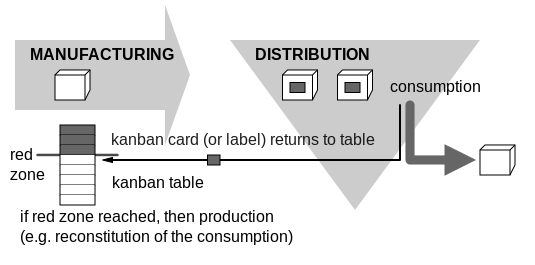
\includegraphics[scale=0.5]{img_kanban}
    \caption{Kanban Paradigm} 
\end{center}
\end{figure}

\begin{figure}[htbp]
\begin{center}
    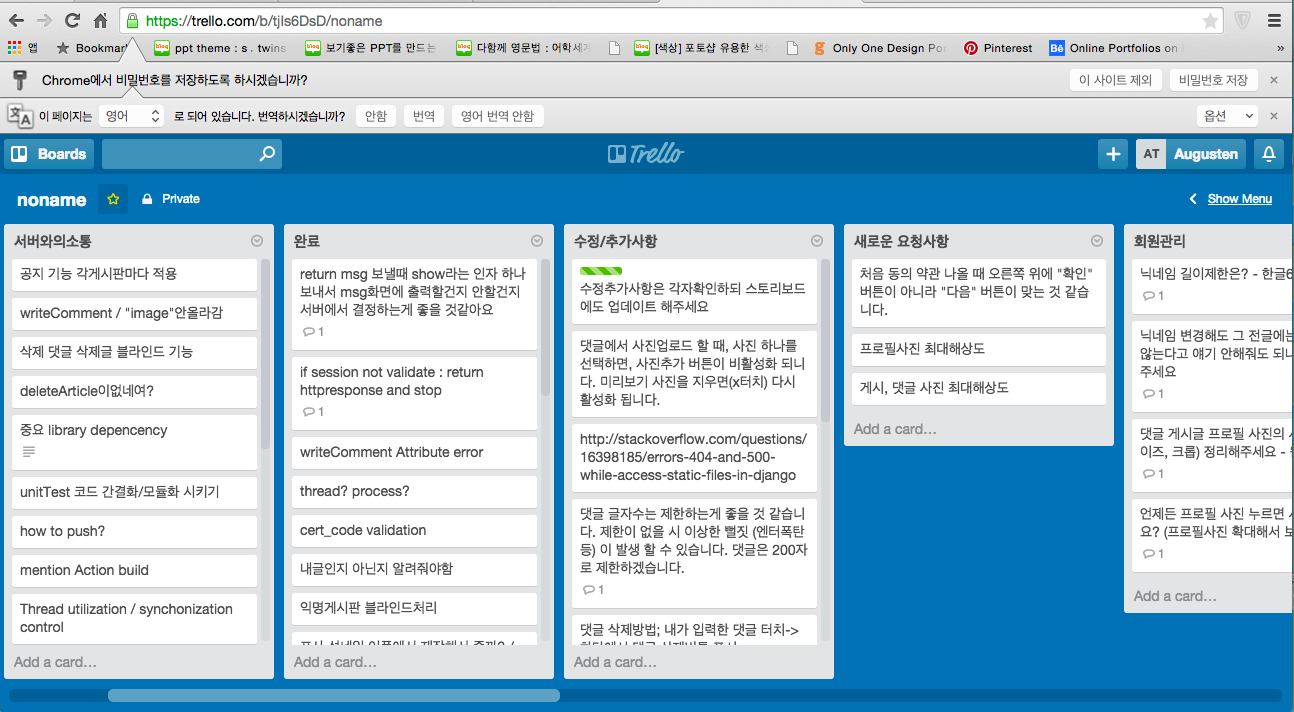
\includegraphics[scale=0.2]{img_trello}
    \caption{trello} 
\end{center}
\end{figure}

Trello is a free web-based project management application. Trello uses the kanban paradigm for managing project. 
Kanban is a scheduling system for lean and just-in-time (JIT) production. \\

Projects are represented by boards, which contain lists (corresponding to task lists). Lists contain cards (corresponding to tasks). Cards are supposed to progress from one list to the next (via drag-and-drop), for instance mirroring the flow of a feature from idea to implementation. Users can be assigned to cards. Users and boards can be grouped into organizations.\\
 




There is a little similar software in Korea, “전시보GO” But this software service is only for big exhibition so small exhibition artist or students can’t use that services. 


3. Task distribution (If you want, you can provide this later at the next phase - design) 

Which member is responsible for what? \\\\\\\\\\\\\\\\\\\\\\\\\\\\





\section{Specifications}
\subsection{Modeling for Specifications \\}


\begin{figure}[htbp]
\begin{center}
    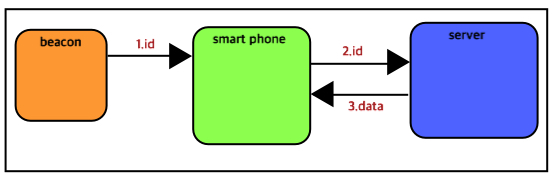
\includegraphics[scale=0.4]{img_01.jpg}
    \caption{basic structure} 
\end{center}
\end{figure}


\quad Beacon sends a specific ID value to the smart phone, when smart phone comes into it?s signal area. Then smart phone application recognizes this ID value and sends this value to server. Server which has this ID value check the location of beacon. After that, server sends the information or data about exhibition to smart phone.\\\\

\subsection{Prototype for Specifications}
\quad Our application is divided into two parts. One is server side with Amazon Web Service EC2 and
Ruby on Rails. The other part is client side acting at the smart phone. Client side, smart phone application, is structured by objective-C (iOS application), and java(Android application)\\\\\\\\\\\\\\\\\\\\\\\\\\\\\\\\\\\\\\

\subsection{Specification for front-end application pages\\}
\quad 0) BLE seraching outside the application\\
\begin{figure}[htbp]
\begin{center}
    
\includegraphics[scale=1]{img_BLE}
    \caption{Information Page02} 
\end{center}
\end{figure}

[BLE]

In our application, there is the service class [SearchBLE.java] which is searching the [BLE]. This service searches the BLE, if the bluetooth module on the smartphone is on. BLE(Bluetooth low energy) is a wireless personal area network(PAN) technology. It is designed and marketed for applications in the healthcare, fitness, security, home entertainment industries, and [beacon].\\

\begin{figure}[htbp]
\begin{center}
    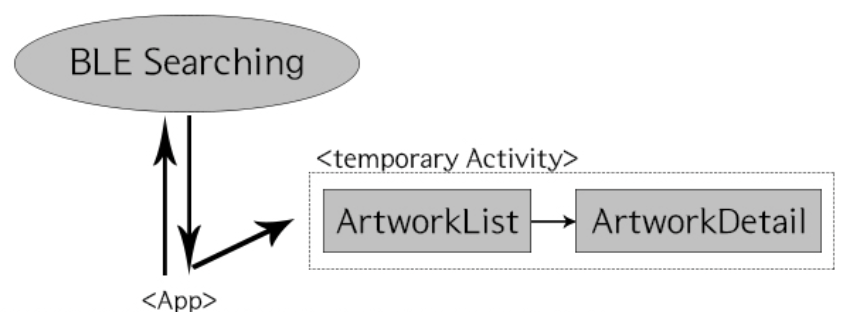
\includegraphics[scale=0.35]{img_tempAct}
    \caption{how temporary activity is operating} 
\end{center}
\end{figure}


If user let bluetooth module [on], smartphone will be searching BLE automatically. That is, it is searching beacon signal. If it finds beacon signal, smartphone get [beacon id]. And smartphone sends this beacon id to server, then server sends to smartphone the all data about exhibition which is stored at that beacon id. After, every data about exhibition is downloaded to smartphone. This downloaded data is showed through [Temporary Activity]. \\

The first page has the brief explains for exhibition and the list of artworks (similar with [My History Page02]). Among these artworks, if you pick one, you can show the details of that artworks such like photos and detail explanations (similar with [My History Page 03]).\\

You have to know this [Temporary Activity] is totally different page with main application. This is [only] temporary. This activity cannot access to main application, and also main application cannot access this activity neither. This activity is only for showing the data from the server. And in main application, not every data showed at temporary activity is stored. Only the name of exhibition and the downloaded date are stored. \\\\\\\\

\quad 1) My history page\\

\begin{figure}[htbp]
\begin{center}
    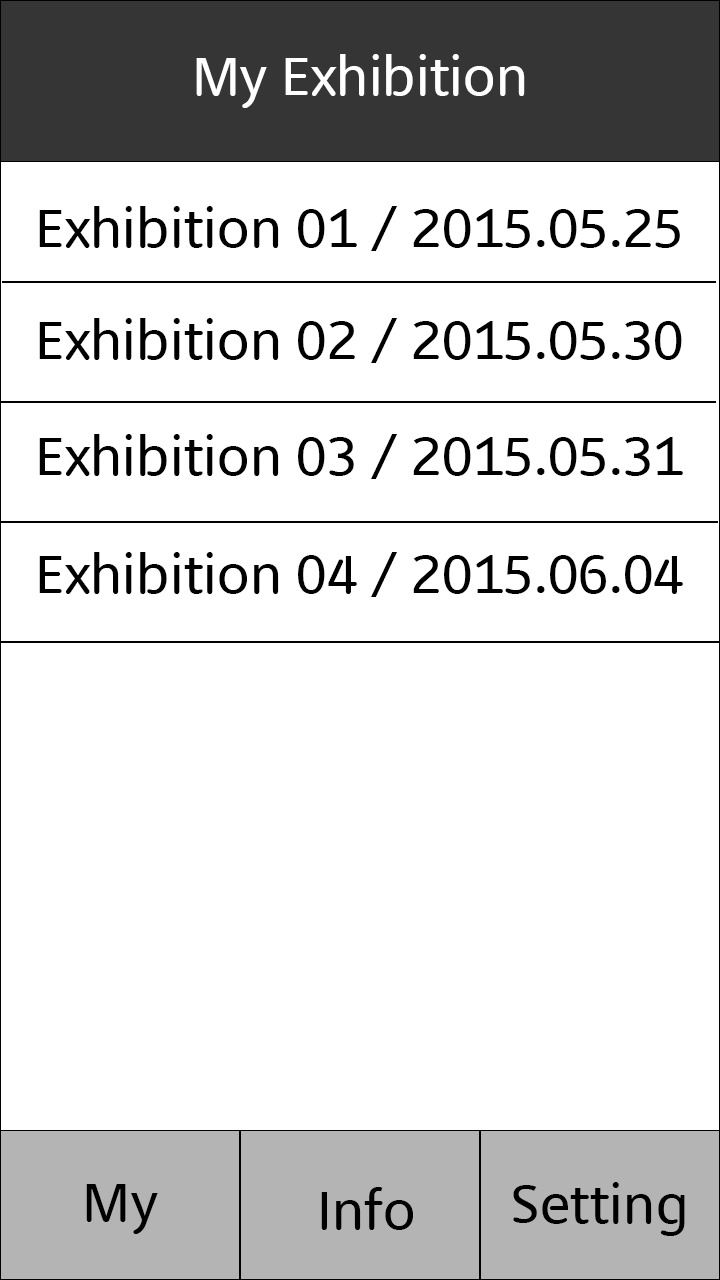
\includegraphics[scale=0.2]{img_My01}
    \caption{BLE} 
\end{center}
\end{figure}


[My History Page01]

This is the first page of application. And you can access this page by tab menu under the display. There is the list of exhibitions which user have already seen.  \\

\begin{figure}[htbp]
\begin{center}
    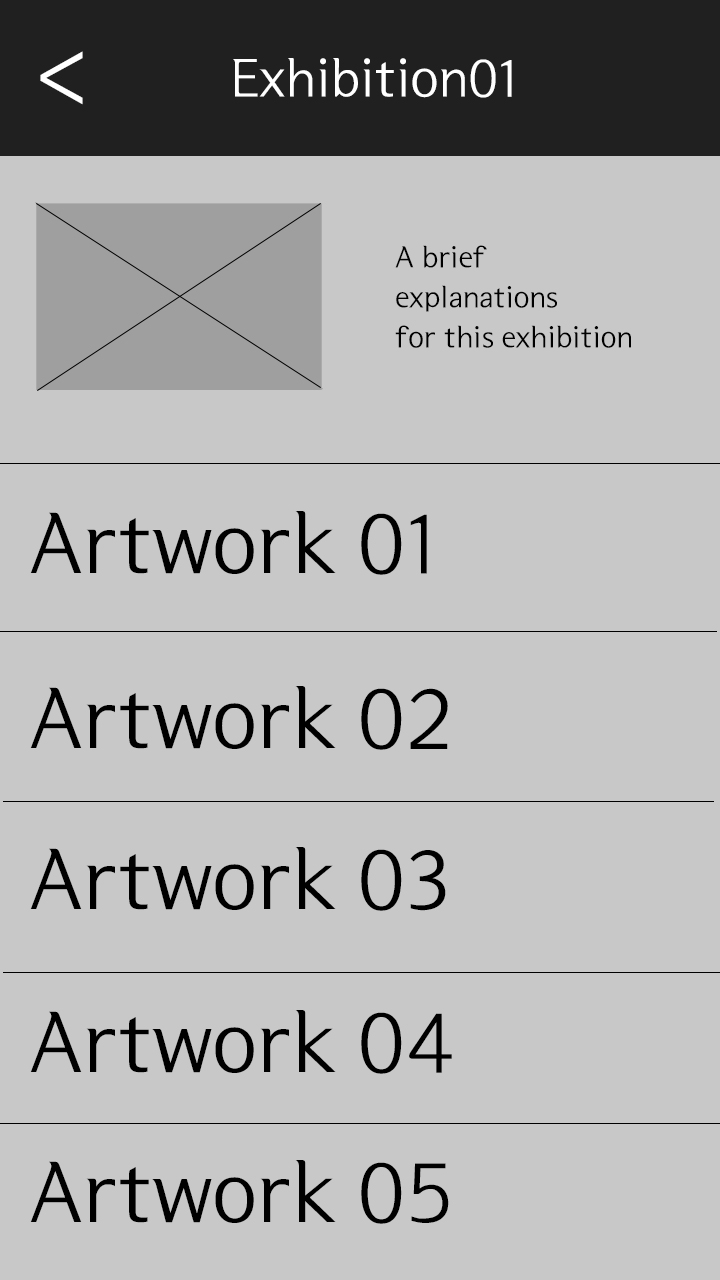
\includegraphics[scale=0.2]{img_exhiDetail01}
    \caption{My History Page02} 
\end{center}
\end{figure}

[My History Page02] 

This is the detail page of the exhibition01. To access this page, applications has to communicate with the back-end server. Server will send the data of Exhibition 01 which the user already downloaded by beacon communication at that Exhibition. On Navigation bar, there is the name of the exhibition. Under the navigation bar, the left side of the first cell,  there is main image of exhibition. And Next to the main image, the right side of the first cell, there is the brief explanation for this exhibition. There will be the information of this exhibition such like the theme of exhibition, the name of exhibition center, address of exhibition center. Below First cell, there is the list of artwork which is displayed in this exhibition.  user can see the detail information about the artwork such as image of artwork, text explanation of artist, or voice-audio explanation. \\\\

\begin{figure}[htbp]
\begin{center}
    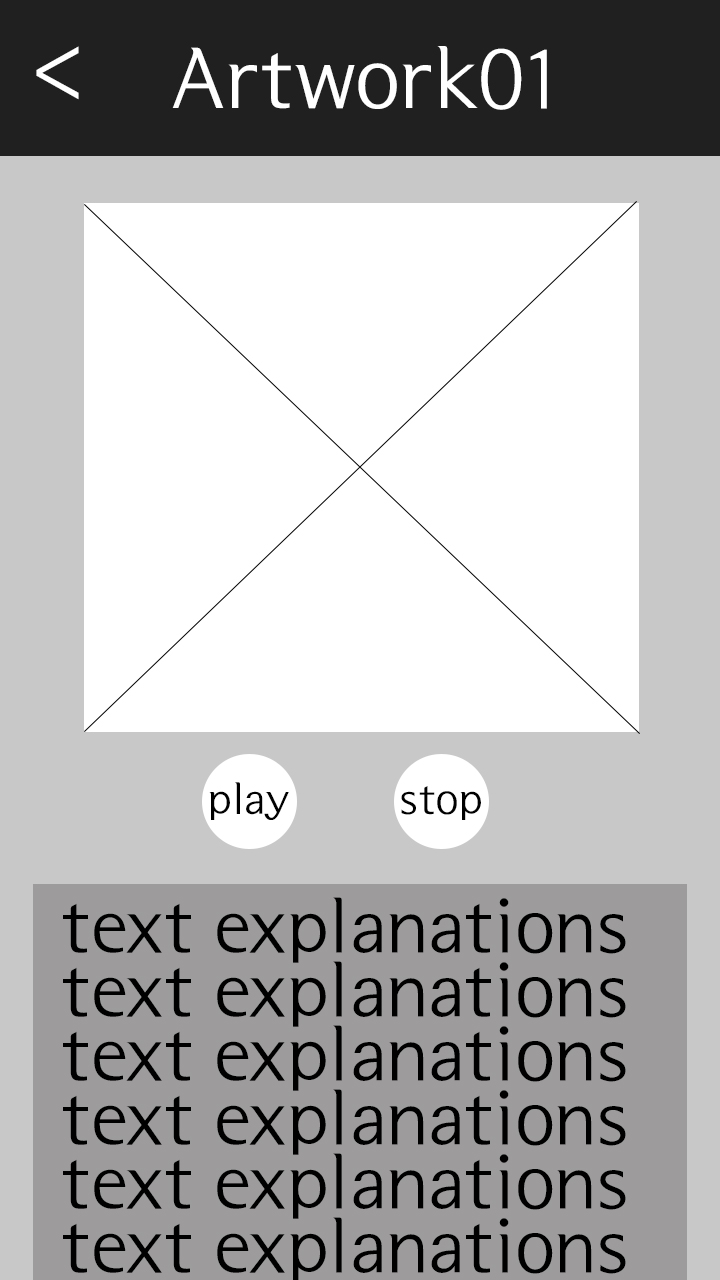
\includegraphics[scale=0.2]{img_exhiDetail02}
    \caption{My History Page03} 
\end{center}
\end{figure}

[My History Page03]

This is the detail page of artwork. On the Navigation bar, there is the name of artwork. Under the Navigation bar, there is the Image of the artwork(If user touch the small image, the pop up window will appear, and user can see the big size image). Below the artwork image, there is the play and stop button. This button is for voice-audio explanation. Voice-audio explanation is not for every artwork. We offer the voice-audio explanation only for the artwork that artist want, and artwork that artist offer the voice-audio explanation data. So if there is the voice-audio explanation, there will be play and stop buttons. And if there is no voice-audio explanation, the play and stop buttons will not exist. Under the Image and buttons, there is the text explanations that artist offer. \\\\\\\\\\\\\\\\\\
\quad 2) Information page\\

\begin{figure}[htbp]
\begin{center}
    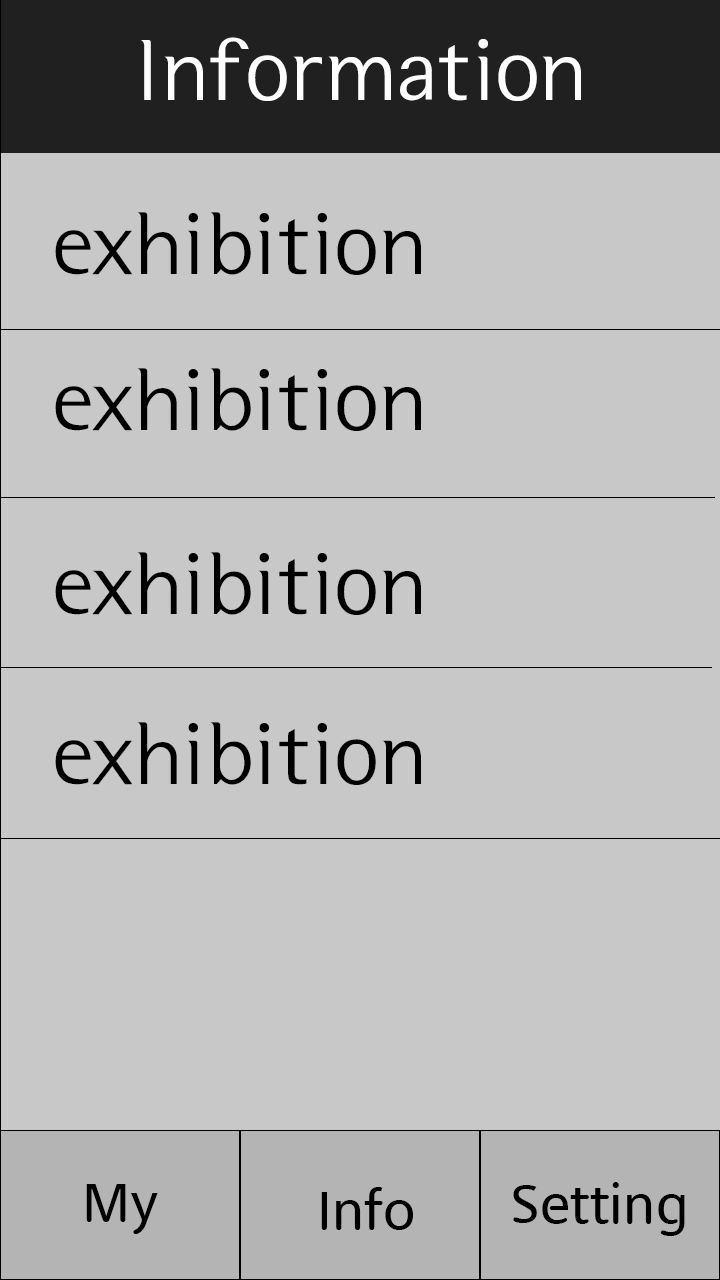
\includegraphics[scale=0.2]{img_Info01}
    \caption{Information Page01} 
\end{center}
\end{figure}

[Information Page01]

user can access the Information page by touching tab menu button under the screen. When user touch the [Info] button under the display, every data is downloaded from server. This page is for noticing the exhibition. There is the list of the exhibitions which is on going now or which will be started. user can check the detail information about the exhibition that user like by touching the name of the exhibition. \\\\\\\\\\\\\\\\\\\\\\\\\\\\

\begin{figure}[htbp]
\begin{center}
    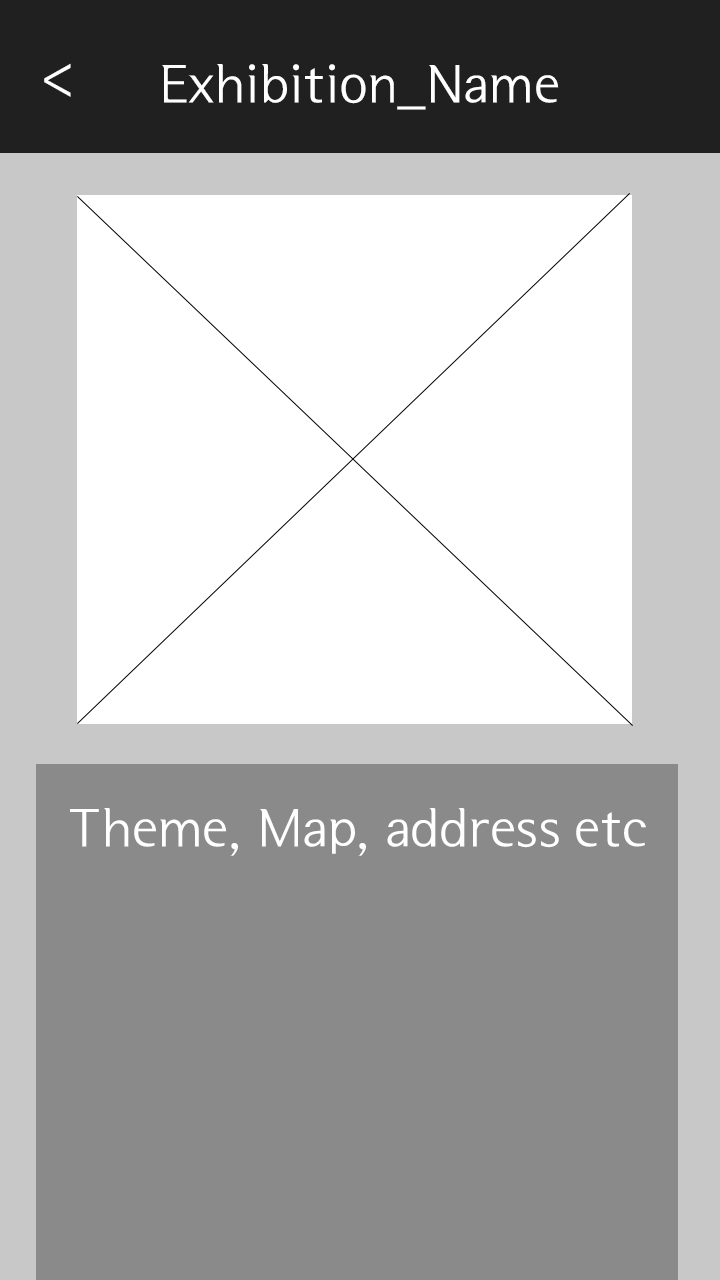
\includegraphics[scale=0.2]{img_infoDetail}
    \caption{Information Page02} 
\end{center}
\end{figure}

[Information Page02]

This page shows the detail information of the exhibition. user can move to the exhibition list page by back button on the navigation bar. On navigation bar, there is the name of the exhibition. Below the navigation bar, user can find the brief information about the exhibition such as the main image of the exhibition, theme of the exhibition, and map or address of exhibition. \\\\\\\\\\\\\\\\\\\\\\\\\\\\\\\\\\



\quad 3) Setting page

\begin{figure}[htbp]
\begin{center}
    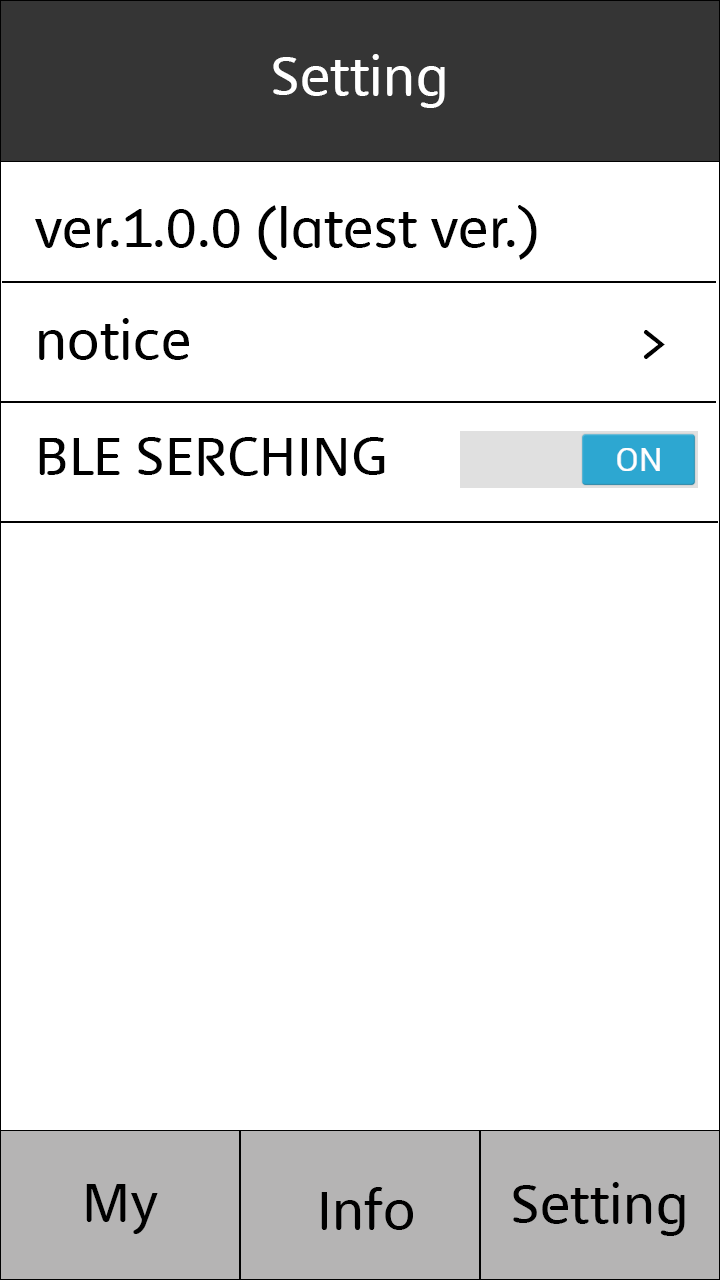
\includegraphics[scale=0.2]{img_setting01}
    \caption{Setting Page} 
\end{center}
\end{figure}

[Setting Page]

In Setting page, there will be the additional function. For example, there will be the on/off button that control the searching BLE. If the user makes the button-state [on], smartphone will search beacon signal and get beacon id ( explained and [0)BLE searching outside the application]). And if user makes the button-state [off], smartphone will not search any beacon signal outside the application. And there will be another board for inform the latest version or notice etc. \\\\\\\\\\\\\\\\\\\\\\\\\\
\subsection{Specifications for Server}


\section{Architecture Design and Implementation}

.\\\\\\\\\\\\\\\\\\\\\\\\\\\\\\\\\\\\\\\\\\\\\\\\\\\\\\\\\\\\\\\\\\\\\\\\\\\\\\\\\\\\\\\\\\\\\\\\\\\\\\\\\\\\\\\\\\\\\\\\\\\\\\\\\\\\\\\\\\\\\\\\\\\\\\\\\\\\\\\\\\\\\\\\\\\\\\\\\\\\\\\\\\

\section{Use Cases}

\begin{figure}[htbp]
\begin{center}
    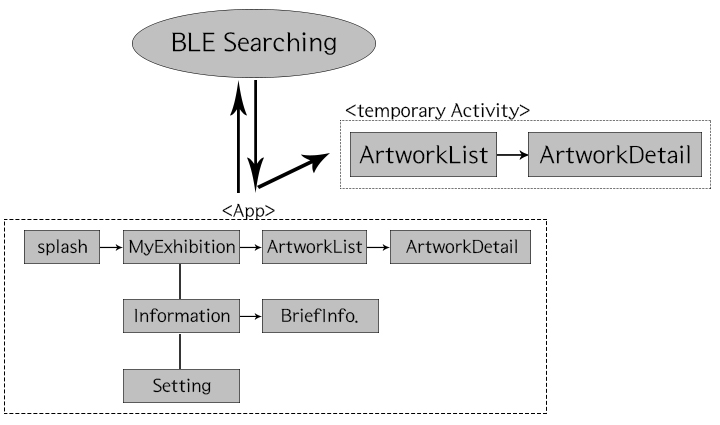
\includegraphics[scale=0.75]{img_flowchart}
    \caption{Beacon Page03} 
\end{center}
\end{figure}

.\\\\\\\\\\\\\\\\\\\\\\\\\\\\\\\\\\\\\\\\\\\\\\\\\\\\\\\\\\\\\\\\\\\\\\\\\\\\\\\\\\\\\\\\\\\\\\\\\\\\\\\\\\\\\\\\\\\\\\\\\\\\\\\\\\\\\\
\quad6-1) BLE searching and push notice
\begin{figure}[htbp]
\begin{center}
    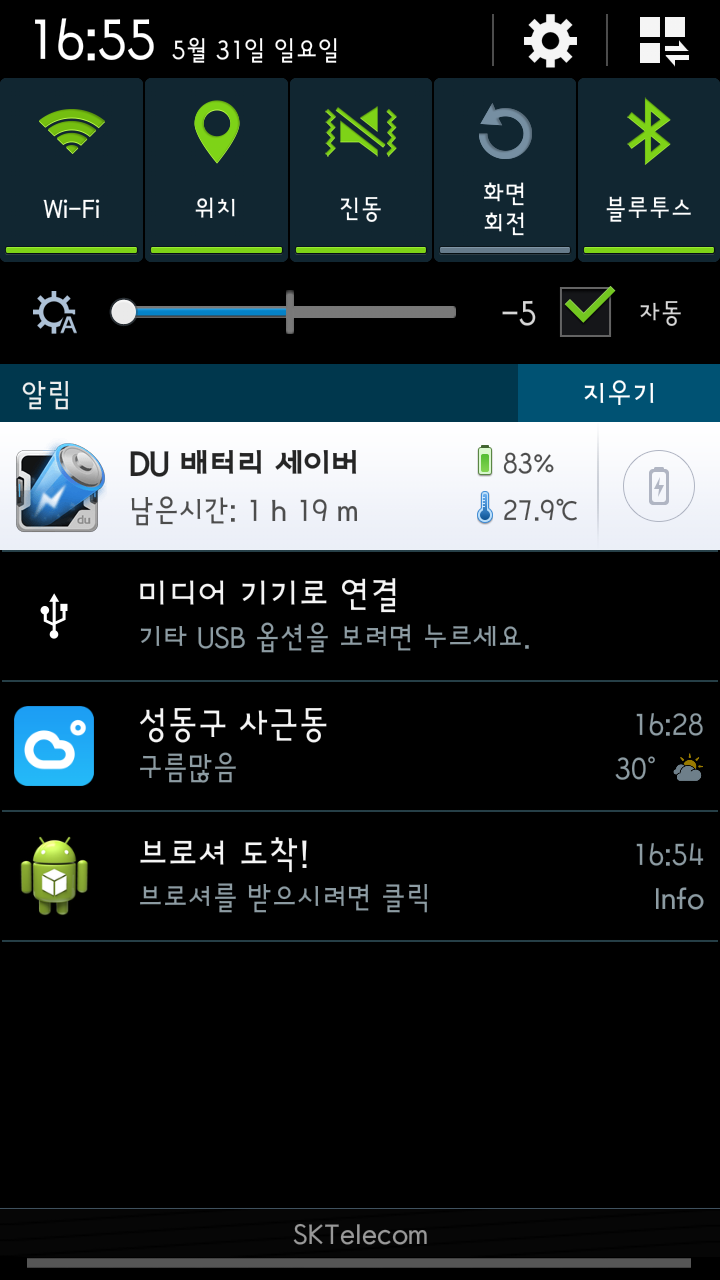
\includegraphics[scale=0.2]{img_capture01}
    \caption{BLE searching and push notice} 
\end{center}
\end{figure}\\
\quad If User turn on the bluetooth module, smartphone finds the BLE signal, and then Server sends to notice that information data about Exhibition is downloaded. If user touch the push notice, then temporary activity is open.\\\\\\\\\\\

\quad6-2) Temporary Activity01 \\
\begin{figure}[htbp]
\begin{center}
    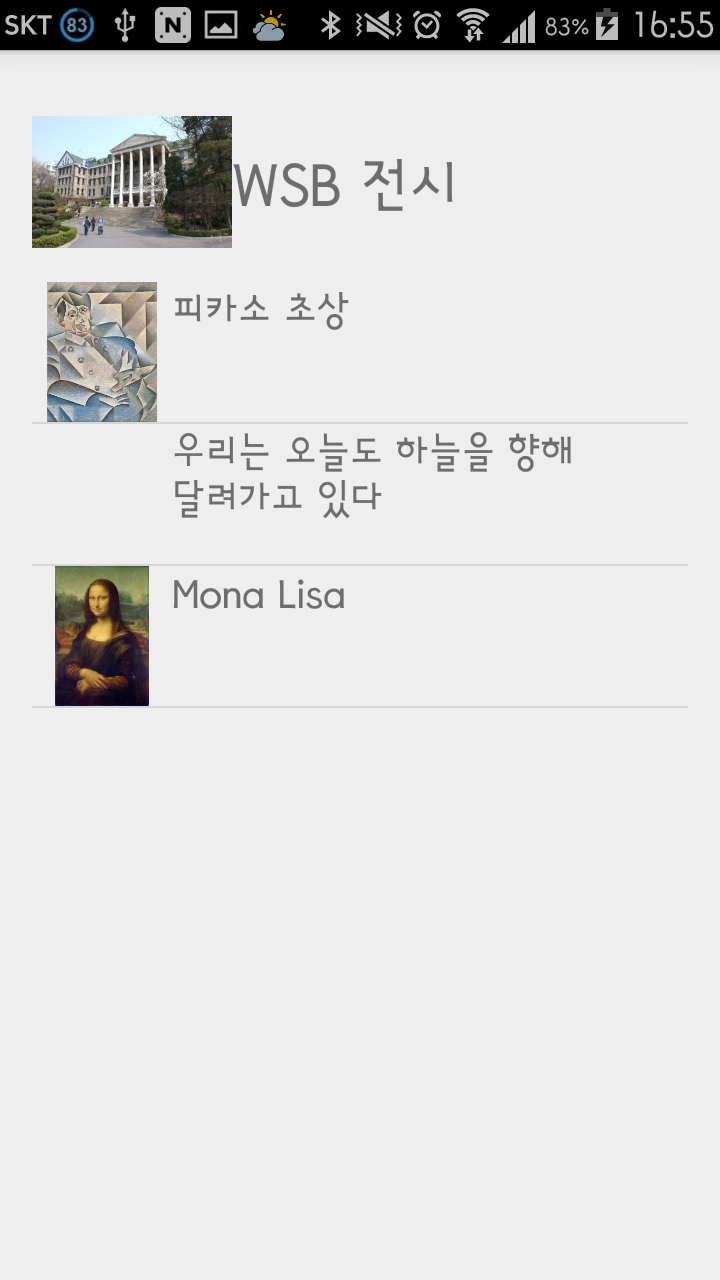
\includegraphics[scale=0.2]{img_capture02}
    \caption{Temporary Activity 01} 
\end{center}
\end{figure}\\
\quad This is the page when temporary page is open. It shows the information received from server. Upper-side of the page, there are the name and main image of exhibition. Under, there are the artwork lists which are displayed at the exhibition now user is seeing.\\\\\\\\\\\\\\

\quad6-2) Temporary Activity02 \\
\quad If the user touch one artwork, he can watch the detail of artwork. Of course every data is received from server. There are image, name, and detail descriptions of the artwork. 
\begin{figure}[htbp]
\begin{center}
    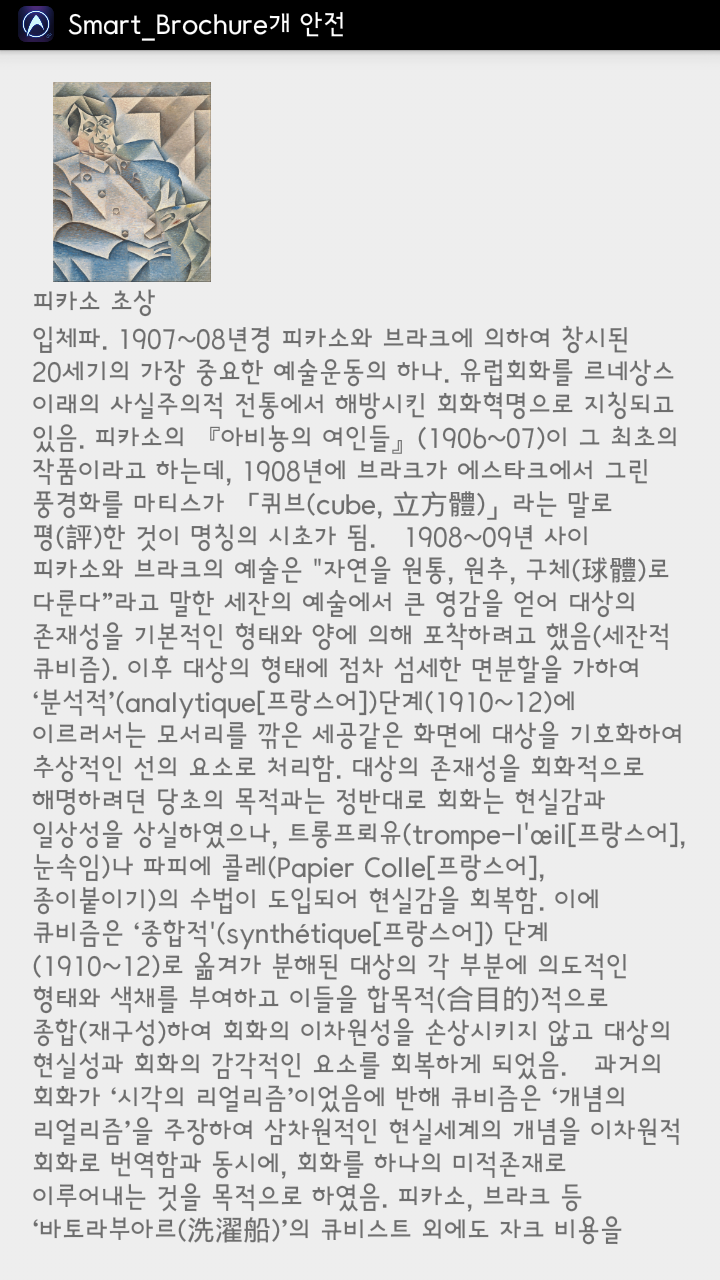
\includegraphics[scale=0.18]{img_capture03}
    \caption{Temporary Activity02} 
\end{center}
\end{figure}
\\\\\\\\

\quad6-3) Main Application - My History Page01\\
\begin{figure}[htbp]
\begin{center}
    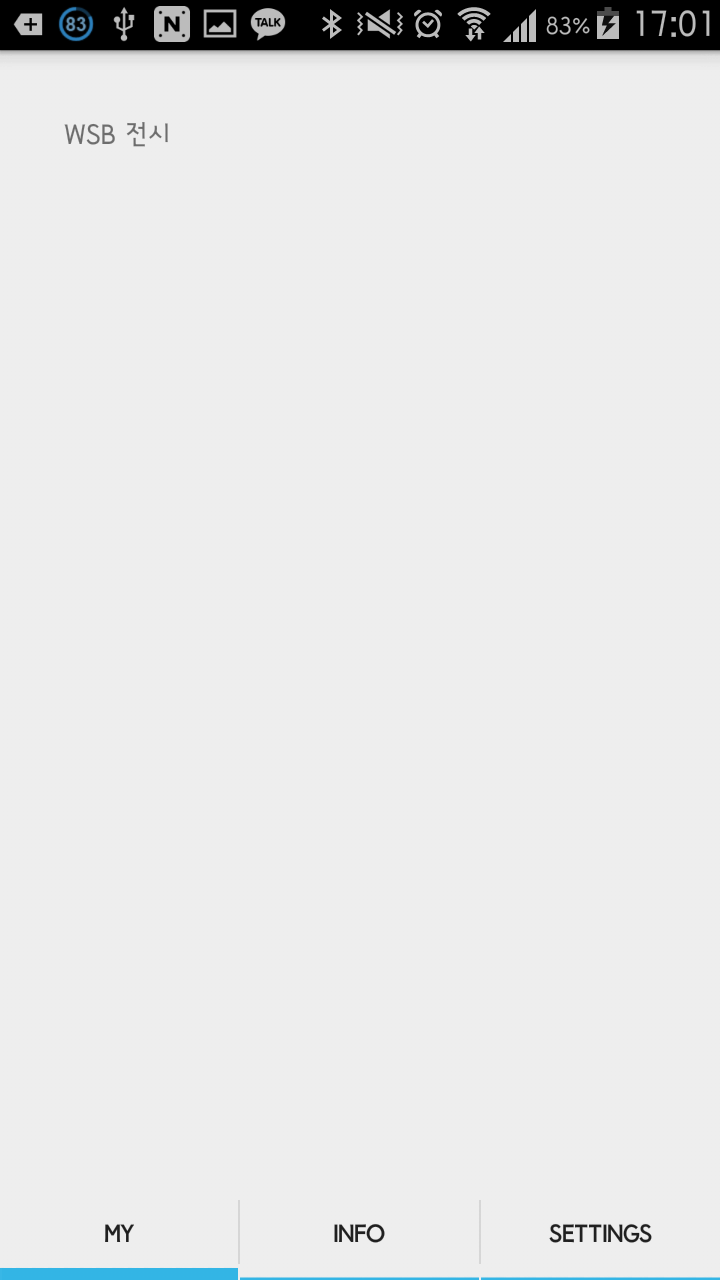
\includegraphics[scale=0.2]{img_capture04}
    \caption{My History01} 
\end{center}
\end{figure}\\
\quad User will see this page when he run the application. It is the first page of main application. First, there is tab menu under the screen. By this tab menu, user can move to page he want to see.  This page is for user own. The data which he received from server and saw through temporary activity is stacked at this page. \\\\\\\\

\quad6-3) Main Application - My History Page02\\
\begin{figure}[htbp]
\begin{center}
    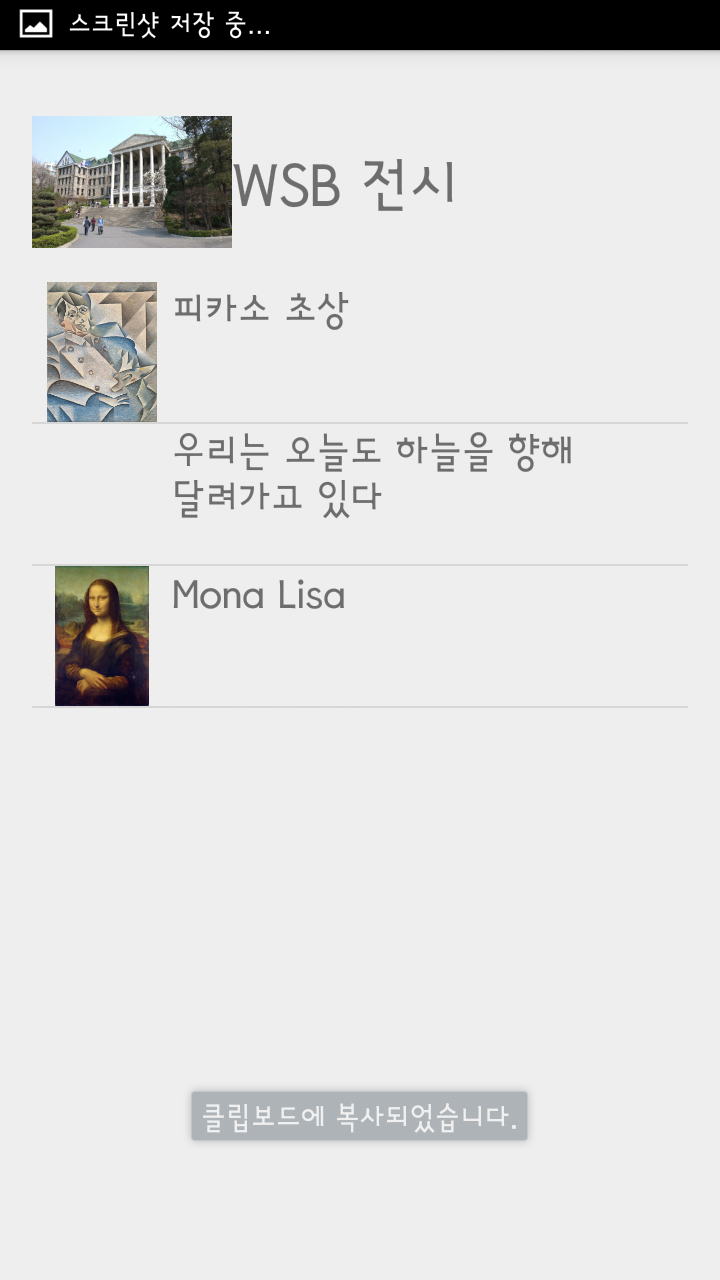
\includegraphics[scale=0.2]{img_capture05}
    \caption{My History02} 
\end{center}
\end{figure}\\
\quad This page shows the detail information about the exhibition. User can see the brief details about the exhibition theme, the Artist, and the list of artwork which is displayed on that exhibition. \\\\\\\\

\quad6-3) Main Application - My History Page03\\
\begin{figure}[htbp]
\begin{center}
    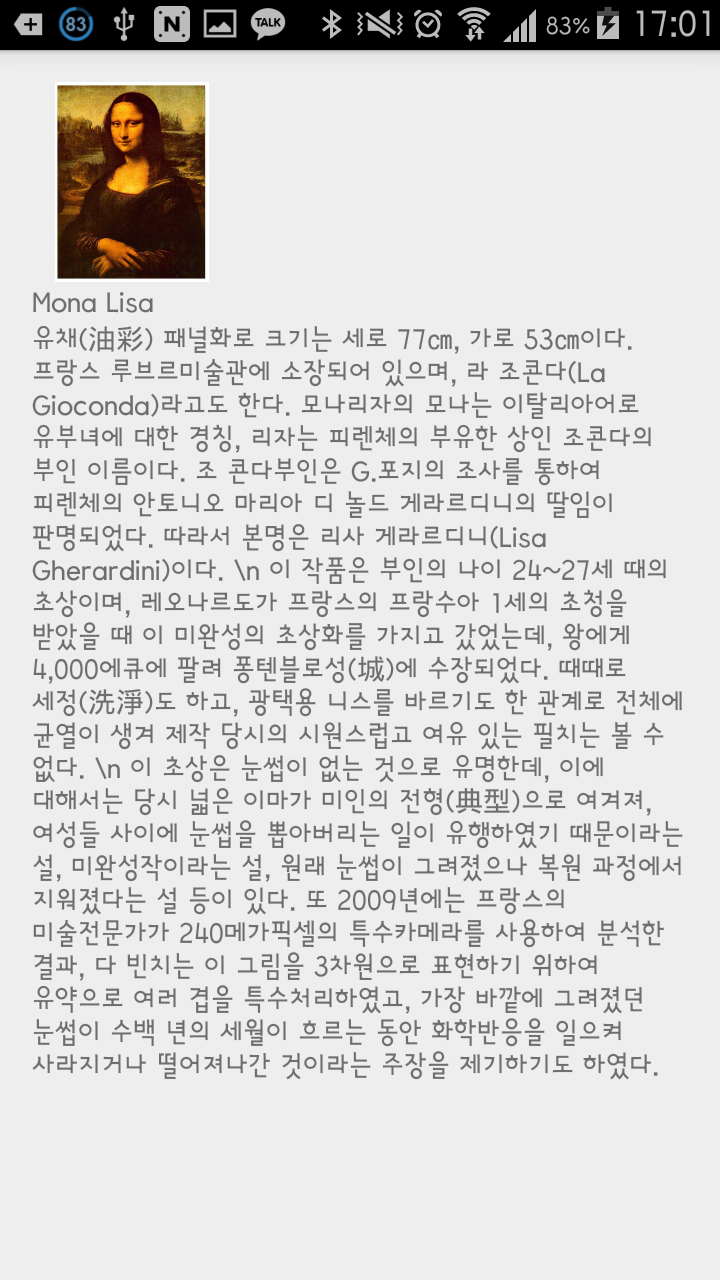
\includegraphics[scale=0.2]{img_capture06}
    \caption{My History03} 
\end{center}
\end{figure}\\
\quad If user touch any artwork at the My History Page01, user can see the detail information about that artwork like this page.\\\\\\\\

\quad6-3) Main Application - Information Page
\begin{figure}[htbp]
\begin{center}
    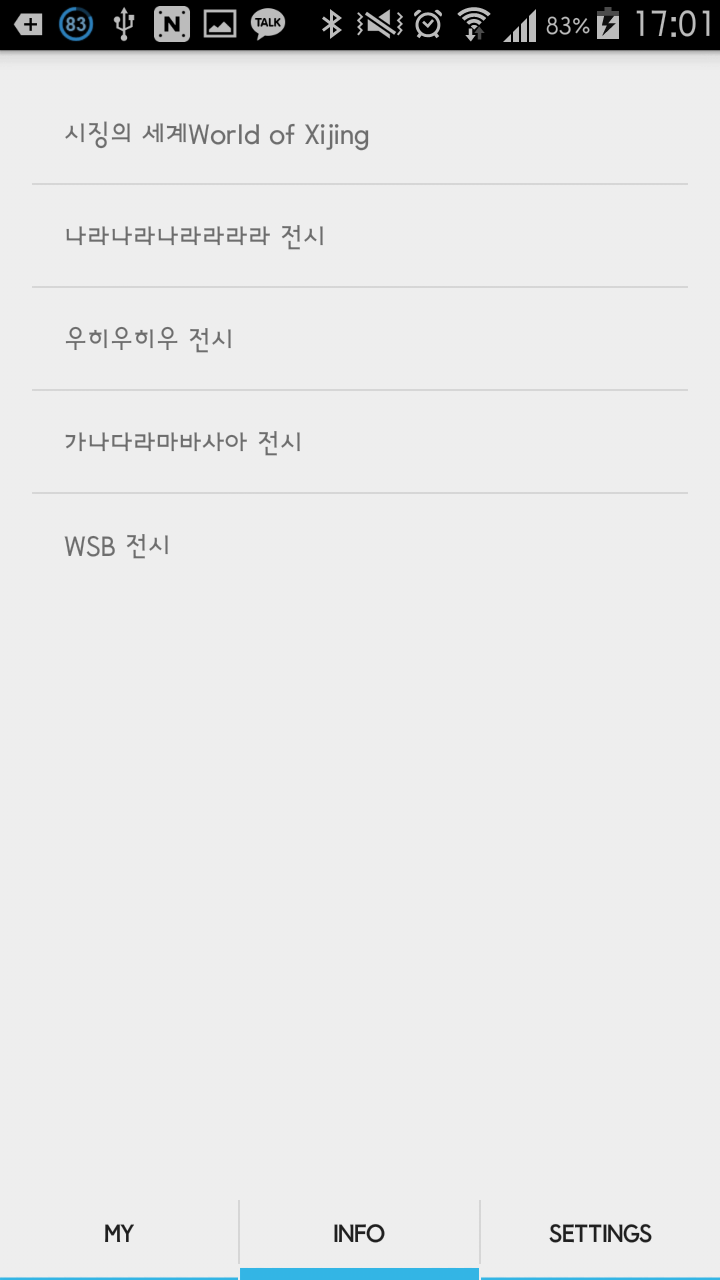
\includegraphics[scale=0.2]{img_capture07}
    \caption{Information Page01} 
\end{center}
\end{figure}

This is the second menu page of the application. User can move to this page from the other using tab menu under the screen. This page is for inform about the other exhibition. On the screen, there will be the list of exhibition that user has not seen yet. If user touch the INFO menu from other page, or swipe down the list, then application connect to the server and get the data of the list of the exhibition. It means, user can refresh the list whenever he wants.\\\\\\\\

\begin{figure}[htbp]
\begin{center}
    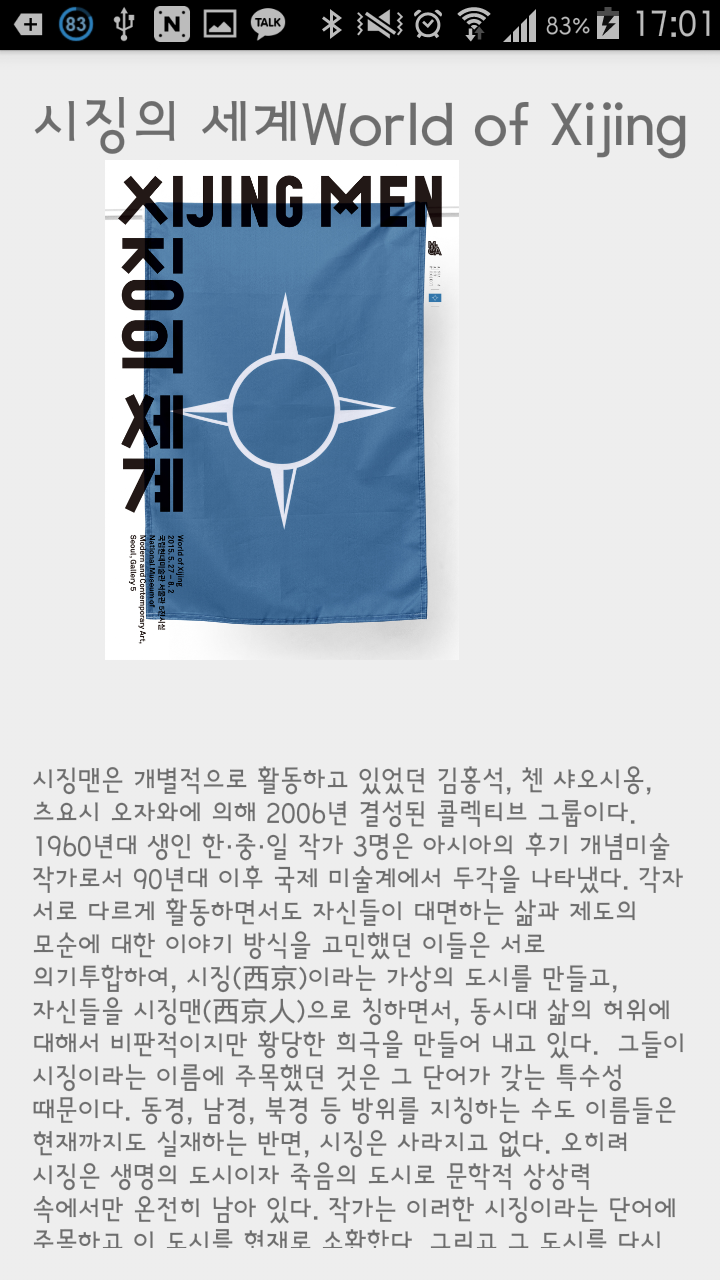
\includegraphics[scale=0.2]{img_capture08}
    \caption{Information Page02} 
\end{center}
\end{figure}

If user select one exhibition, he can see the detail information about that exhibition such like the main image of the exhibition, information about the artist, the address of the exhibition and so on. \\\\\\\\

\quad6-3) Main Application - Setting Page
\begin{figure}[htbp]
\begin{center}
    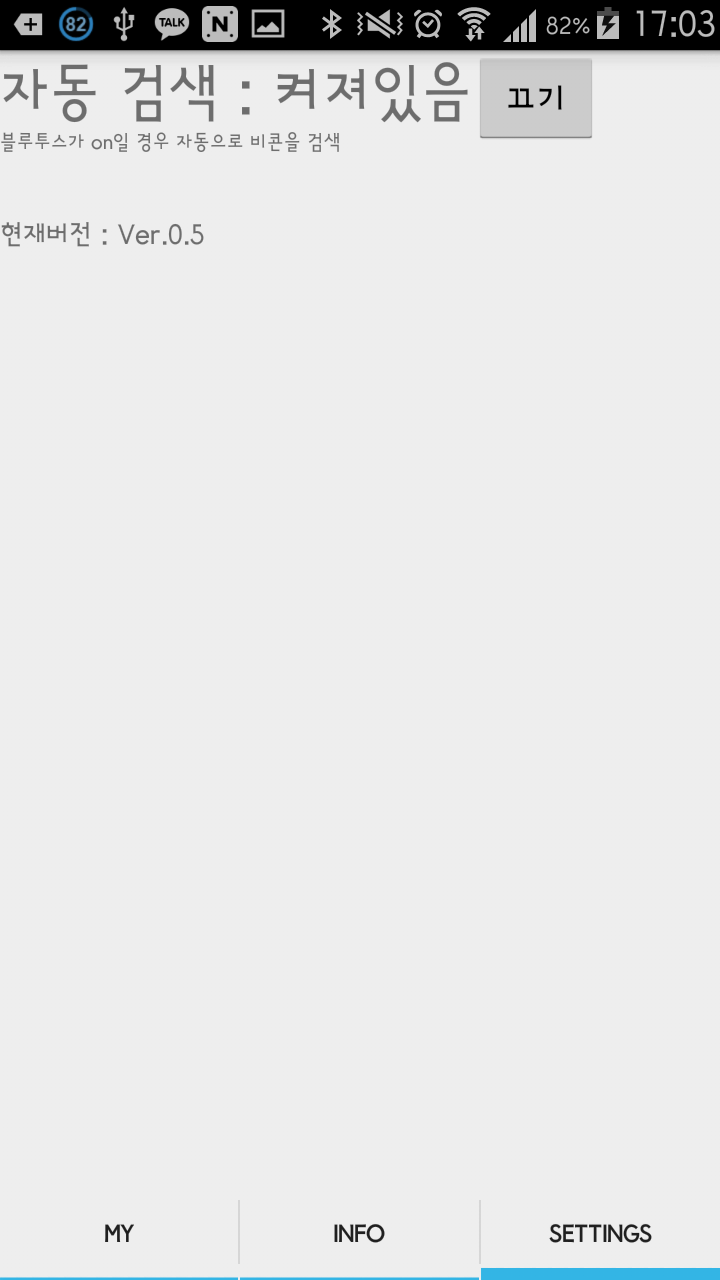
\includegraphics[scale=0.2]{img_capture09}
    \caption{Setting Page01} 
\end{center}
\end{figure}

User can turn on or off the function searching the BLE. - Turn on\\\\\\\\

\begin{figure}[htbp]
\begin{center}
    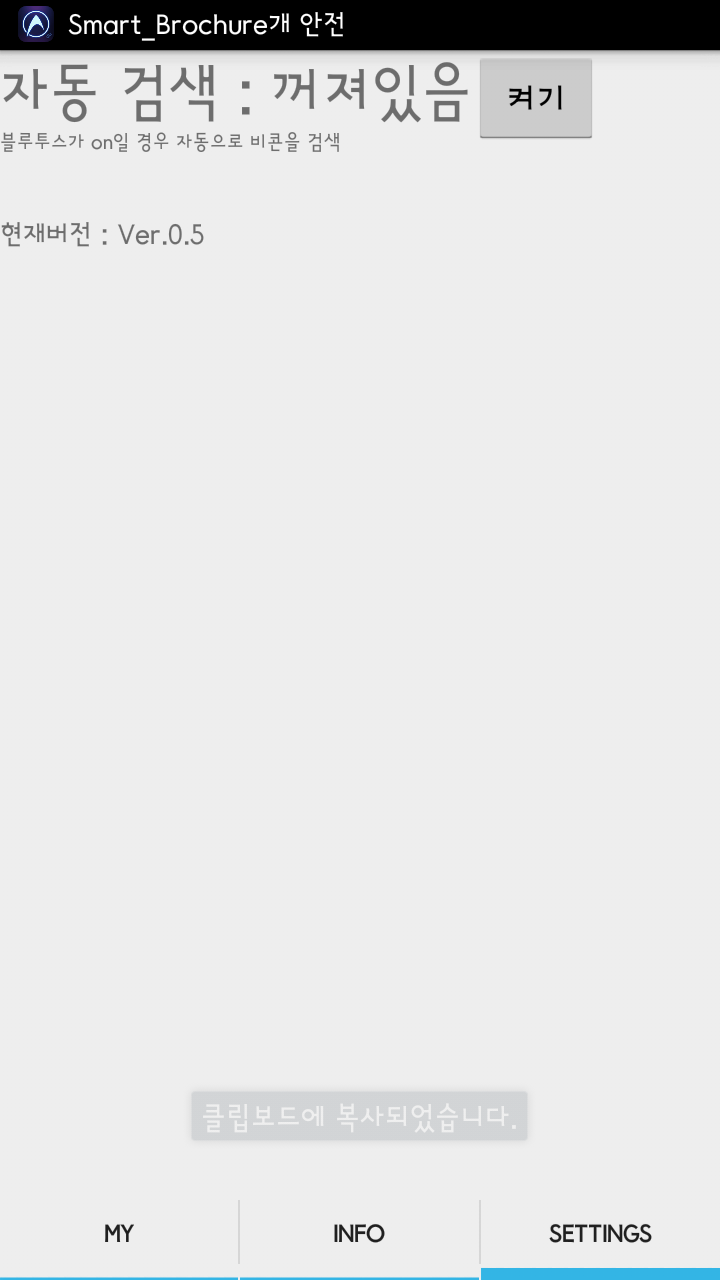
\includegraphics[scale=0.2]{img_capture10}
    \caption{Setting Page02} 
\end{center}
\end{figure}

User can turn on or off the function searching the BLE. - Turn off\\\\\\\\
.
% An example of a floating figure using the graphicx package.
% Note that \label must occur AFTER (or within) \caption.
% For figures, \caption should occur after the \includegraphics.
% Note that IEEEtran v1.7 and later has special internal code that
% is designed to preserve the operation of \label within \caption
% even when the captionsoff option is in effect. However, because
% of issues like this, it may be the safest practice to put all your
% \label just after \caption rather than within \caption{}.
%
% Reminder: the "draftcls" or "draftclsnofoot", not "draft", class
% option should be used if it is desired that the figures are to be
% displayed while in draft mode.
%
%\begin{figure}[!t]
%\centering
%\includegraphics[width=2.5in]{myfigure}
% where an .eps filename suffix will be assumed under latex, 
% and a .pdf suffix will be assumed for pdflatex; or what has been declared
% via \DeclareGraphicsExtensions.
%\caption{Simulation Results}
%\label{fig_sim}
%\end{figure}

% Note that IEEE typically puts floats only at the top, even when this
% results in a large percentage of a column being occupied by floats.


% An example of a double column floating figure using two subfigures.
% (The subfig.sty package must be loaded for this to work.)
% The subfigure \label commands are set within each subfloat command, the
% \label for the overall figure must come after \caption.
% \hfil must be used as a separator to get equal spacing.
% The subfigure.sty package works much the same way, except \subfigure is
% used instead of \subfloat.
%
%\begin{figure*}[!t]
%\centerline{\subfloat[Case I]\includegraphics[width=2.5in]{subfigcase1}%
%\label{fig_first_case}}
%\hfil
%\subfloat[Case II]{\includegraphics[width=2.5in]{subfigcase2}%
%\label{fig_second_case}}}
%\caption{Simulation results}
%\label{fig_sim}
%\end{figure*}
%
% Note that often IEEE papers with subfigures do not employ subfigure
% captions (using the optional argument to \subfloat), but instead will
% reference/describe all of them (a), (b), etc., within the main caption.


% An example of a floating table. Note that, for IEEE style tables, the 
% \caption command should come BEFORE the table. Table text will default to
% \footnotesize as IEEE normally uses this smaller font for tables.
% The \label must come after \caption as always.
%
%\begin{table}[!t]
%% increase table row spacing, adjust to taste
%\renewcommand{\arraystretch}{1.3}
% if using array.sty, it might be a good idea to tweak the value of
% \extrarowheight as needed to properly center the text within the cells
%\caption{An Example of a Table}
%\label{table_example}
%\centering
%% Some packages, such as MDW tools, offer better commands for making tables
%% than the plain LaTeX2e tabular which is used here.
%\begin{tabular}{|c||c|}
%\hline
%One & Two\\
%\hline
%Three & Four\\
%\hline
%\end{tabular}
%\end{table}


% Note that IEEE does not put floats in the very first column - or typically
% anywhere on the first page for that matter. Also, in-text middle ("here")
% positioning is not used. Most IEEE journals/conferences use top floats
% exclusively. Note that, LaTeX2e, unlike IEEE journals/conferences, places
% footnotes above bottom floats. This can be corrected via the \fnbelowfloat
% command of the stfloats package.





% conference papers do not normally have an appendix


% use section* for acknowledgem



% trigger a \newpage just before the given reference
% number - used to balance the columns on the last page
% adjust value as needed - may need to be readjusted if
% the document is modified later
%\IEEEtriggeratref{8}
% The "triggered" command can be changed if desired:
%\IEEEtriggercmd{\enlargethispage{-5in}}

% references section

% can use a bibliography generated by BibTeX as a .bbl file
% BibTeX documentation can be easily obtained at:
% http://www.ctan.org/tex-archive/biblio/bibtex/contrib/doc/
% The IEEEtran BibTeX style support page is at:
% http://www.michaelshell.org/tex/ieeetran/bibtex/
%\bibliographystyle{IEEEtran}
% argument is your BibTeX string definitions and bibliography database(s)
%\bibliography{IEEEabrv,../bib/paper}
%
% <OR> manually copy in the resultant .bbl file
% set second argument of \begin to the number of references
% (used to reserve space for the reference number labels box)




% that's all folks
\end{document}


